You can install the client on any machine in the network, and then install the \gdagent on various other machines in the network. 

This scenario is shown in the following diagram (\bxfigref{diffmachines}). 

\begin{figure}
\begin{center}
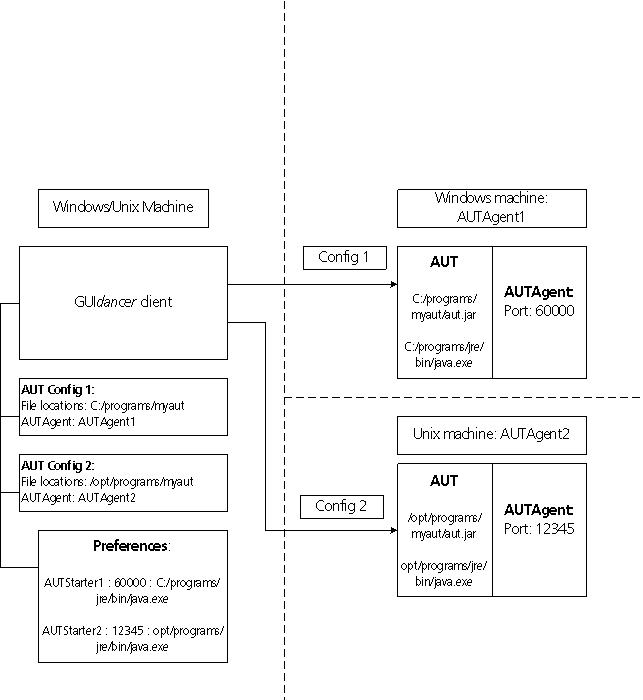
\includegraphics{Concepts/Architecture/PS/diffmachines}
\caption{\app{} architecture}
\label{diffmachines}
\end{center}
\end{figure}

Within the \app{} client, you can define configurations for your \gdaut{}. The configurations specify where \app{} should look for the \gdaut{} jar or exe file, the JRE binary etc., and on which machine it should look.

\app{} lets you specify different \gdagent{} hosts and port numbers to connect to. 

